\section{La Via Lattea}\label{sec:via-lattea}
\begin{figure}
    \centering
    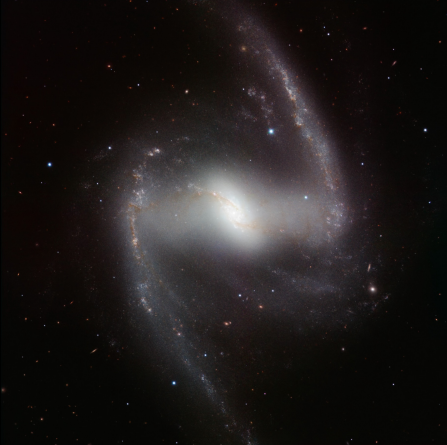
\includegraphics[width = 0.5\textwidth]{immagini/via-lattea.png}
    \caption{La nostra galassia, la Via Lattea.}
    \label{fig:via-lattea}
\end{figure}

La Via Lattea è una galassia a spirale, come si può vedere in figura~\ref{fig:via-lattea}; alcuni studi sembrano confermare che ci sia anche una barra nella nostra galassia, quindi pensiamo possa essere classificata come SBc. 

\subsection{Proprietà generali}
Di seguito riportiamo i dati principali relativi alla Via Lattea.

\subsubsection{Dimensioni}
Il diametro del disco è $\sim 30 kpc$. Se consideriamo però l'intero ammasso globulare (quindi l'alone attorno al disco) arriviamo a un diametro $\sim 100 kpc$.

\subsubsection{Massa}
La massa totale è $\sim 10^{12} \si{\solarmass}$, di cui circa il 90\% è massa di materia oscura e il restante 10\% è invece materia barionica. 
La massa del bulge è invece $\sim 10^{10} \si{\solarmass}$, quindi è un circa $1/6$ della massa totale del disco.

La materia barionica può a sua volta essere divisa nelle sue componenti per analizzare la massa di ognuna di queste:
\begin{itemize}
    \item Le stelle, che stanno soprattutto nel disco, hanno una massa pari a $\sim 5 \cdot 10^{10} \si{\solarmass}$.
    \item Anche il gas si trova soprattutto nel disco e abbiamo che la sua massa abbonda a $\sim 5 \cdot 10^9 \si{\solarmass}$; il gas è all'80\% idrogeno neutro monoatomico (HI) e al 20\% idrogeno molecolare (H$_{2}$). 
    \item La polvere ha una massa di $\sim 3 \cdot 10^7 \si{\solarmass}$ e la troviamo nell'intero spazio occupato dalla galassia.
\end{itemize}

Come abbiamo detto il gas si trova soprattutto nel disco ma c’è evidenza del gas nell’alone. L’origine della sua presenza nell'alone è ancora ignota, ci sono due ipotesi a proposito:
\begin{itemize}
    \item La prima ipotesi è che il gas sia di origine interna. Infatti le supernovae possono creare una "superbolla" di gas ionizzato; questa può poi esplodere ed emettere il gas ionizzato. A sua volta questo non può allontanarsi lateralmente, ma solo radialmente dalla stella stessa e quindi può poi ricadere sul disco, dando luogo al fenomeno della cosiddetta \emph{fontana galattica}. Questa potrebbe essere quindi una prima spiegazione della presenza di gas diffuso nell'alone.
    \item La seconda ipotesi è che invece questo gas sia di origine esterna; ad esempio potrebbe essere gas proveniente da galassie che sono state cannibalizzate dalla nostra galassia o potrebbe essere gas primordiale in caduta sulla nostra galassia (assieme a dei filamenti di materia oscura).  Questa ipotesi di origine esterna del gas potrebbe aiutare a comprendere il processo di formazione stellare all'interno del disco, altrimenti difficile da spiegare.
\end{itemize} 

\subsubsection{Luminosità}
La magnitudine assoluta su tutta la banda V è $M_V = -20.5$. La galassia emette in tutto lo spettro secondo i dati riportati in tabella~\ref{tab:luminosita-via-lattea}. Come possiamo vedere la banda di emissione dominante è proprio la banda ottica.

\begin{table}[!ht]
    \caption{Luminosità della Via Lattea nello spettro.}
    \label{tab:luminosita-via-lattea}
    \centering
    \begin{tabular}{ll}
    \toprule
    Spettro &  Luminosità \\
    \midrule
    Radio & $3 \cdot 10^{38}$ \si{erg}/\si{s}\\
    IR & $3 \cdot 10^{41}$ \si{erg}/\si{s}\\
    Ottico & $3 \cdot 10^{43}$ \si{erg}/\si{s}\\
    Raggi X & $3 \cdot 10^{40}$ \si{erg}/\si{s}\\
    Raggi $\gamma$ & $3 \cdot 10^{38}$ \si{erg}/\si{s}\\
    \bottomrule
    \end{tabular}
\end{table}

\subsubsection{Rotazione}
La velocità differenziale di rotazione della galassia a una distanza pari a quella del Sole è pari a $v_{rot} \sim 225 \;\si{km}/\si{s}$. Il periodo di rotazione di conseguenza risulta essere $P_{rot} \sim 250 \; \si{Myr}$.

\subsubsection{Posizione del Sole}
Il Sole si trova a una distanza di $\sim 8 \;\si{kpc}$ dal centro della galassia e si trova a circa $8 \;\si{pc}$ sopra rispetto al piano galattico (piano su cui appoggia la galassia a spirale).

\subsection{Popolazione stellare nella Via Lattea} \label{pop-stellare-via-lattea}
\begin{figure}
    \centering
    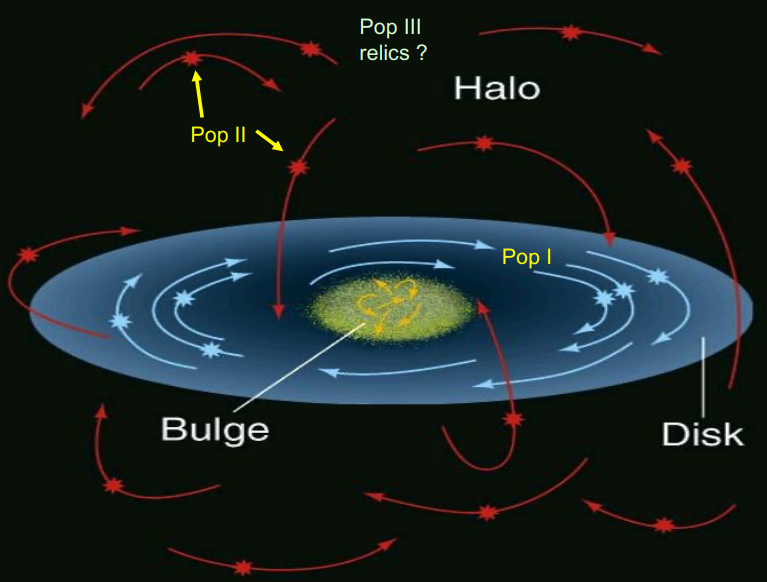
\includegraphics[width = 0.5 \textwidth]{immagini/popolazione-stellare-via-lattea.png}
    \caption{Popolazione stellare nella Via Lattea.}
    \label{fig:popolazione-stellare-via-lattea}
\end{figure}
Le stelle interne alla nostra galassia sono di diverso tipo (possiamo vedere uno schema riassuntivo in figura~\ref{fig:popolazione-stellare-via-lattea}:
\begin{itemize}
    \item \emph{Popolazione I}: Le stelle che appartengono a questa categoria sono giovani (hanno un'età che va da $\sim \si{Myrs} - 10 \;\si{Gyrs}$) e percorrono orbite quasi circolari sul piano della galassia (a questa categoria appartiene anche il Sole). Inoltre sono caratterizzate da una metallicità\footnote{La metallicità è definita come $Z = 1-X-Y$, dove $X$ e $Y$ sono rispettivamente le concentrazioni in massa di idrogeno ed elio; per il sole si ha $Z_{\odot}\sim 0.02$} variabile, con $Z=0.01-0.04$. 
    \item \emph{Popolazione II}: Le stelle di questa popolazione sono più vecchie (hanno un'età di $\sim 12 - 13.5 \; \si{Gyrs}$) e compiono orbite eccentriche (quindi sono stelle molto veloci). In più sono composte da un bulge più ricco di metalli ($Z \leq 2$) e un alone stellare con una bassa metallicità ($Z < 0.002$).
    \item \emph{Relitti Popolazione III}: Sembra che siano presenti anche dei relitti di oggetti di popolazione III; queste stelle sono estremamente vecchie (con un età $> 13 \; \si{Gyrs}$) e fin'ora sono state scoperte alcune stelle con una bassissima metallicità che sarebbero compatibili con questi oggetti di Popolazione III (vengono dette \emph{extremly metal poor}, EMP, $Z < 10^{-3} \;Z_{\odot}$).
\end{itemize}

Un'altra caratteristica molto importante da notare è legata invece alla polvere: fra noi e il bulge della galassia è presente molta polvere che assorbe molta luminosità (si dice che il bulge è oscurato in direzione radiale). Addirittura 1 fotone su $10^{12}$ arriva a noi e ciò rende molto difficile il suo studio, motivo per cui il bulge è la regione che conosciamo meno. Ciò nonostante però la tecnologia ci aiuta, quindi tramite telescopi che aggiustano l'immagine (si parla di ottica adattiva) siamo in grado di eliminare la sbrodolatura dovuta alla nostra atmosfera e in parte alla polvere stellare. 

\subsection{Il buco nero al centro della Via Lattea}
Negli anni 70 è inoltre stato scoperto che al centro della nostra galassia è presente un buco nero supermassiccio, chiamato Sagittarius A* (è stato conferito a Reinard Genze e Andrea Ghez il premio Nobel per la fisica 2020 proprio per questa scoperta). Si è riusciti ad arrivare a questa conclusione analizzando le traiettorie delle singole stelle vicine al centro della galassia e utilizzando la terza legge di Keplero: 
\begin{equation*}
    G(M_{BH} + m) = \frac{4\pi^2}{P^2}a^3
\end{equation*}
In questo modo si è determinato che $M_{BH} \sim 3 \cdot 10^6 \;\si{\solarmass}$.

La presenza di un buco nero al centro della nostra galassia è in realtà una caratteristica comune di molte galassie; infatti in molti casi si osserva la presenza di un centro gravitazionale nelle galassie dalle traiettorie delle stelle, che però non emette radiazione e quindi non è osservabile. La conclusione dopo vari anni di osservazione è che effettivamente si tratta proprio di un buco nero.

\subsection{Interazioni fra la Via Lattea e altre galassie}
Esistono alcune missioni spaziali che hanno il compito di osservare tutto il cielo per svariati anni e a diverse lunghezze d’onda; si chiamano "all sky survey" e sono in grado di restituirci la più larga e precisa mappa 3D della nostra galassia (ad es. Gaia, missione dell'ESA). Grazie a queste missioni si sono scoperte sovradensità di stelle "coerenti" dal punto di vista cinematico e chimico che riteniamo siano ciò che rimane dopo diverse interazioni con altre galassie satellite più piccole. In particolar modo in figura~\ref{fig:interazioni-via-lattea} possiamo vedere le varie correnti stellari che possiamo interpretare come i resti delle galassie satellite cannibalizzate dalla Via Lattea, quindi sono praticamente uno storico dell'evoluzione della Via Lattea. Un esempio scoperto nel 2003 di questo fenomeno è la galassia ellittica nana del Sagittario, che si trova a $\sim 15 \si{kpc}$ dal centro della nostra galassia. Analizzando un'orbita ricostruita si può vedere che questa galassia ha già attraversato il piano della Via Lattea svariate volte in passato; ora sembra destinata ad attraversare il nostro disco galattico  e infine ad essere inglobata dalla nostra galassia.

\begin{figure}
    \centering
    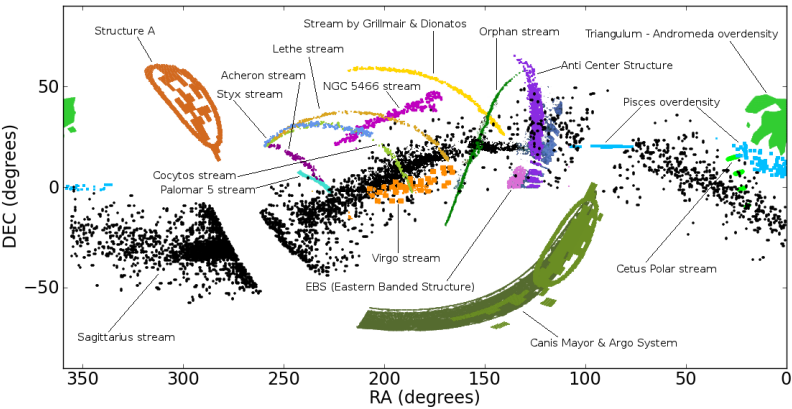
\includegraphics[width = 0.8\textwidth]{immagini/interazioni-via-lattea.png}
    \caption{Correnti stellari che indicano precedenti interazioni fra la Via Lattea e galassie satellite.}
    \label{fig:interazioni-via-lattea}
\end{figure}